\chapter{Progress}

\section{Project progress}
The project has two parts, currently, the progress is at the point of discovering and implementing machine learning for modeling the arbiter PUF. Methods such as reinforcement learning
and graph attention neural network(so-called GAT) were used. First, the type of reinforcement learning that was implemented is the SARSALambda Q learning \cite{Reference9}. The general idea is that an agent will 
explore the environment with a final goal by randomly choosing actions space and recording the rewards. 

Assuming Figure \ref{fig:figure11} is the PUF environment, a red and green circle is the starting point for top path and bottom path, each black rectangle represents a multiplexer with unique delay and the yellow 
circle is the goal. There are three actions: going up, going down and going straight. The reward of the multiplexer is determined by the delay, the bigger the delay, the smaller the reward, vice versa. In the training phase, 
the agent will travel through different combinations of multiplexers and construct a Q table(See Table \ref{tab:table1}) by collecting rewards on multiplexers. The final goal for the agent is to find the route with 
the lowest delay. After the training, when selecting a CRPs, and inputting the challenge to the agent, ideally, the agent can calculate, compare two paths' reward and reply the correct response. For example, assume 
a challenge 00001 has response 1(which means the bottom path is faster), the calculation operation is:
\begin{equation}
    Challenge(00001) =\begin{cases}
    0.082+0.008+0.041+0.002+0.07 = 0.203, & \text {Top path: 1,3,5,7,10}.\\
    0.022+0.415+0.222+0.555+0 = 1.214, & \text {Bottom path: 2,4,6,8,9}.
    \end{cases}
\end{equation}

\begin{equation}
    0.203 < 1.214, \text { return response: 1}.
\end{equation}
In general, the route with lower delay will have a higher reward, on the other hand, the route with higher delay will have a lower reward. If the agent can predict with high accuracy, the arbiter PUF's CRPs pattern can say to 
be successfully modelled. However, the accuracy for this modeling is around 60\% - 69\%, which is not a satisfying result. The problem can be the following: not providing enough features, the exploration does not 
cover every possible route, etc.

\begin{figure}[htp]
    \centering
    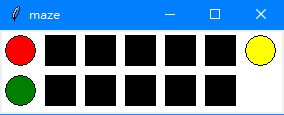
\includegraphics[width=6cm]{figures/figure11.jpg}
    \caption{SARSALambda Q learning example environment}
    \label{fig:figure11}
    \end{figure}

\begin{table}[ht]
    \center
    \begin{tabular}{c|ccc}
    Multiplexer & go up & go down & go straight\\
    \hline
    1 & 0.000 & 0.028 & 0.082\\
    2 & 0.094 & 0.000 & 0.022\\
    3 & 0.000 & 0.357 & 0.008\\
    4 & 0.009 & 0.000 & 0.415\\
    5 & 0.000 & 0.181 & 0.041\\
    6 & 0.042 & 0.000 & 0.222\\
    7 & 0.000 & 0.641 & 0.002\\
    8 & 0.003 & 0.000 & 0.555\\
    9 & 0.000 & 0.070 & 0.000\\
    10 & 0.000 & 0.000 & 0.131\\
    \end{tabular}
    \caption{Q table for example environment}
    \label{tab:table1}
    \end{table}

As for the GAT \cite{Reference10}, the basic idea of the GAT is that each node aggregate the neighbours’ features based on adjacency matrix, adjacency attention value then update each node's features. 
The updated features will insert into the neural network and perform the classifying task. In order to reach high accuracy, the main task for the GAT is to update the adjacency attention matrix to
right value.

For a detail example, look at Figure \ref{fig:figure12}, which is a arbiter PUF structure. Assume each nose in Figure \ref{fig:figure12} represent a multiplexer, and has node feature $f1,f2,f3,f4$. If input a 
challenge 00, a one way relation is defined: 
$m3 \rightarrow m1$, $m4 \rightarrow m2$, including self-loop, and the adjacency matrix can be constructed(See 4.3). 
\begin{equation}
    \begin{blockarray}{ccccc}
    M1 & M2 & M3 & M4\\
    \begin{block}{(cccc)c}
        1 & 0 & 0 & 0 & M1\\
        0 & 1 & 0 & 0 & M2\\
        1 & 0 & 1 & 0 & M3\\
        0 & 1 & 0 & 1 & M4\\
    \end{block}
    \end{blockarray}
    \label{matrix}
\end{equation}

\begin{figure}[htp]
    \centering
    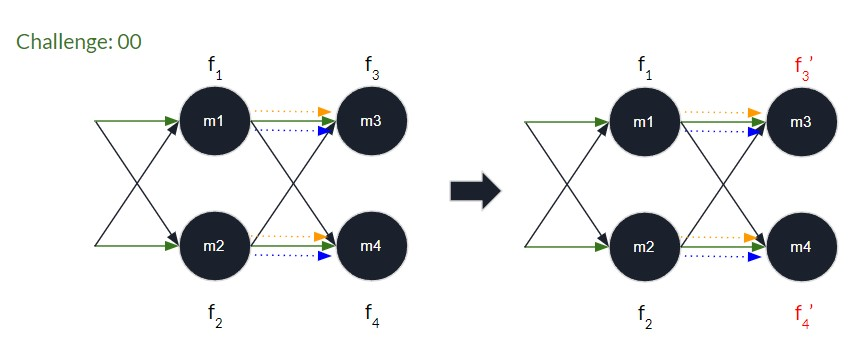
\includegraphics[width=16cm]{figures/figure12.jpg}
    \caption{GAT aggregation}
    \label{fig:figure12}
    \end{figure}

In article \cite{Reference10}, there are four steps to aggregate the features of each node. The first step, add a weight matrix to gain enough expressive power to transform the features into higher-level features:
\begin{equation}
    n_i = \mathcal{W}_if_i
\end{equation}

The second step, calculate a un-normalized attention value between every two nodes(i and j), but only consider nodes that is neighbor of i($j \in N_i$), where $N_i$ is the neighbor of node i that can be observed in 
adjacency matrix(See 4.3). First, concatenates the features of the two nodes(symbol $\Vert$ represent concatenation), then perform a dot product with a trainable weight vector a, and applies a LeakyReLU at last:

\begin{equation}
    c_{ij} = LeakyReLU(\overrightarrow{a}^T(n_i \Vert n_j))
\end{equation}

The third step, apply Softmax function to normalize:
\begin{equation}
    \alpha_{ij} = \frac{exp(e_{ij})}{\sum_{k \in N_i}  exp(e_{ik})} 
\end{equation}

The fourth step, aggregate the updated features from neighbors to current node, and consider the attention matrix:
\begin{equation}
    f_i^{'} = \sigma (\sum_{j \in N_i} \alpha_{ij}n_j)
\end{equation}

After updating every node's features, concatenates the node features of top path($f_1+f_3^{'}$)and bottom path($f_2+f_4^{'}$), and insert into a classify layer. Next, compare the output with ground fact
(response of the challenge) to update the parameter to increase the prediction rate. Ideally, the adjacency matrix will keep updating according to different input challenges, and the GAT will be able to 
learn the pattern after looking at many samples. However, there is doubt that whether the GAT support dynamically changing adjacency matrix, so this idea is not done yet.





